\begin{tikzpicture}
\tikzstyle{box} = [draw,inner sep=7,minimum size=57,line 
		width=1, very thick, draw=black, fill=black!20, text width=100, text centered]
		\tikzstyle{invisible} = [outer sep=0,inner sep=0,minimum size=0]
		\tikzstyle{stealth} = [-stealth, very thick]
	\begin{scope} [scale=0.1, shift={(-112.5,10)}]
		\draw [very thick] (-2,0.5) arc (0:-180:1.5);
		\draw [very thick] (-2,3.5) arc (0:180:1.5);
		\node [invisible] (v1) at (-5,3.5) {};
		\node [invisible] (v3) at (-2,3.5) {};
		\node [invisible] (v2) at (-5,0.5) {};
		\node [invisible] (v4) at (-2,0.5) {};
		\draw [very thick] (v1) edge (v2);
		\draw [very thick] (v3) edge (v4);
		\node [invisible] (v9) at (-5,3) {};
		\node [invisible] (v10) at (-4,3) {};
		\node [invisible] (v11) at (-5,2) {};
		\node [invisible] (v12) at (-4,2) {};
		\node [invisible] (v13) at (-5,1) {};
		\node [invisible] (v14) at (-4,1) {};
		\node [invisible] (v15) at (-2,1) {};
		\node [invisible] (v16) at (-3,1) {};
		\node [invisible] (v17) at (-2,2) {};
		\node [invisible] (v18) at (-3,2) {};
		\node [invisible] (v19) at (-2,3) {};
		\node [invisible] (v20) at (-3,3) {};
		\draw [very thick] (-1.5,0.5) arc (0:-180:2);
		\node [invisible] (v7) at (-3.5,-1.5) {};
		\node [invisible] (v8) at (-3.5,-2.5) {};
		\node [invisible] (v5) at (-5.5,-2.5) {};
		\node [invisible] (v6) at (-1.5,-2.5) {};
		\draw [very thick] (v5) edge (v6);
		\draw [very thick] (v7) edge (v8);
		\draw [very thick] (v9) edge (v10);
		\draw [very thick] (v11) edge (v12);
		\draw [very thick] (v13) edge (v14);
		\draw [very thick] (v15) edge (v16);
		\draw [very thick] (v17) edge (v18);
		\draw [very thick] (v19) edge (v20);
	\end{scope}
\node [box] (v23) at (-3,1) {Adaptación de la tasa de muestreo a $11025 \frac{muestras}{segundo}$};
\node [box] (v22) at (-8.1,1) {Analógico $\xrightarrow{}$ Digital};
\node [invisible] (v21) at (-11,1) {};
\node [box] (v24) at (2.5,1) {FFT de $1024~muestras$};
\node [box, minimum size=40] (v30) at (8.5,2.5) {Módulo};
\node [box, minimum size=40] (v31) at (8.5,-0.5) {Fase};
\node [box] (v26) at (2.5,-4.5) {$mod\cdot e^{j\cdot fase}$};
\node [box] (v27) at (-3,-4.5) {iFFT};
\node [box] (v28) at (-8.1,-4.5) {Analógico $\xleftarrow{}$ Digital};
	\begin{scope}[scale=0.4, shift={(-35.6,-8.15)}, xscale=-1]
	\draw [rounded corners, very thick, fill] (-7,-2.6) node [invisible] (v25) {} -- (-7,-3.6) node [invisible] {} -- (-6.5,-3.5) node [invisible] {} -- (-5.5,-4.5) node [invisible] {} -- (-5.5,-1.5) node [invisible] {} -- (-6.5,-2.5) node [invisible] {} -- (v25);
	\draw [very thick] (-5.0603,-2.658) arc (19.9988:-20:1);
	\draw [very thick] (-4.5905,-2.487) arc (19.9994:-20:1.5);
	\draw [very thick] (-4.1206,-2.316) arc (19.9988:-20:2);
	\draw [very thick] (-3.6508,-2.1449) arc (20.0013:-20:2.5);
	\end{scope}
\node [invisible] (v29) at (-11,-4.5) {};
\node [box, minimum size=40] (v32) at (8.5,-5) {Red neuronal recurrente};
\draw [stealth] (v21) edge node [anchor=south]{$x_{in}(t)$} (v22);
\draw [stealth] (v22) edge node [anchor=south]{$x_{in}(n)$}(v23);
\draw [stealth] (v23) edge node [anchor=south]{$\widetilde{x_{in}}(n)$} (v24);
\draw [stealth,out=0,in=180] (v24) edge node [anchor=north west]{$FFT(n)$} (v30);
\draw [stealth, out=0, in=180] (v24) edge (v31);
\draw [stealth,out=0,in=0] (v30) edge node [anchor=east]{$mod(n)$} (v32);
\draw [stealth] (v32) edge node [anchor=north]{$\widetilde{mod}(n)$} (v26);
\draw [stealth] (v26) edge node [anchor=south]{$imag_(n)$} (v27);
\draw [stealth] (v27) edge node [anchor=south]{$x_{out}(n)$} (v28);
\draw [stealth] (v28) edge node [anchor=south]{$x_{out}(t)$} (v29);
\node [invisible] (v33) at (10.5,-3) {};
\draw [very thick, out=0, in=15] (v31) edge (v33);
\draw [stealth] (v33) edge node [anchor=south]{$fase(n)$} (v26);
\end{tikzpicture}